\chapter{Evaluierung}\label{kap:eval}

\section{Evaluierungs Metriken}\label{sec:metricen}

hier zb confusion matrix, IOU, mAP erklären.

\section{Ergebnisse}\label{sec:results}

\subsection{Modell Vergleich}

hier modelle auf genauigkeit und geschwindig keit vergleichen 
und für nächste abschnitte eins auswählen



\subsection{Regularisierung}\label{subsec:regularization}

\begin{table}[htb]
    \centering
    \label{tab:regularization}
    \begin{tabular}{| l || c | c |} 
        \hline
        Regularisierung & mAP & Loss\\
        \hline
        keine & 1 & 2 \\
        \hline
        Early Stopping & 1 & 2 \\
        \hline
        Augmentierung & 1 & 2 \\
        \hline
        weight decay & 1 & 2 \\
        \hline
    \end{tabular}        
    \caption{Regularization}
\end{table}


ergibt dann zB early stoping und aug sind gleich.
\\
daher wird im nächsten abschnitt geproüft wie sich 
die Modelle für Daten einer anderer Distribution verhalten.


\subsection{Dataset Distributions}\label{subsec:distributions}
Da sowohl trainings als auch eval daten aus dem web bezogen wurden,
also der gleichen distribution sind, diese aber nicht unbedingt 
den realen bedingungen entsprechen, wurde ein weiteres Evaluierungs 
Set mit Eigenen Aufnahmen erstellt, welche, da in der Umgebung 
(Wiltierpark in Reutlingen) aufgenommen, der tatsächlichen daten 
wahrschverteilung eher entspricht.
\\
ergebnisse tabellarisch vergleichen: handy vs orig für die in 
\ref{subsec:regularization} beschriebenen Regularisierungs techniken\\
wenn für Augmentierung besser, heist das Augmentierung ist besser als 
early stopping für robustheit gegenüber umgebung (zb belichtungen)
\\
Die Regularisierungen Early Stopping und Augmentierung wurden 
nun nocheinmal mit einem eigenen Datenset evaluiert und miteinander 
verglichen.


\begin{table}[htb]
    \centering
    \label{tab:regularization}
    \begin{tabular}{| l || c | c | c | c |} 
        \hline
        Regularisierung & $mAP_{orig}$ & $mAP_{handy}$ & $Loss_{orig}$ &  $Loss_{handy}$\\
        \hline
        Early Stopping (100k steps) & 0.6715 & 0.4265 & 0.6742 & 0.267\\
        \hline
        Augmentierung (200k steps) & 0.6914 & 0.4537 & 0.6738 & 0.2503\\ % hier noch verschiedene kombinationen von augmentierungen
        \hline
    \end{tabular}        
    \caption{Regularization}
\end{table}

Wie zu erwarten unterscheiden sich die Loss Werte für das Origiganel 
Eval Set wegen Early stopping nicht sehr. Für die Handy Bilder ist 
der Augmentierungs Loss etwas besser, was auf eine gr robustheit 
gegenüber Daten aus anderer Distribution zurückzuführen ist.

Die mAP Werte sind sowohl für original als auch für handy datenset 
bei Augmentierung deutlich besser, da sich wie in \ref{plot:map_loss} 
der mAP erst später seinem Endwert annähert als der Loss.



\begin{figure}[htb]
    \centering
    \begin{subfigure}{6cm}
        \centering
        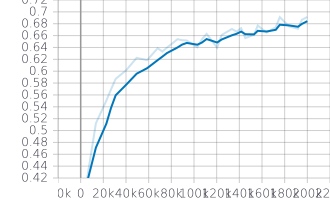
\includegraphics[width=6cm]{./Bilder/eval/mAP.png} % hier die svg graphiken verwenden
        \subcaption{mAP}    
    \end{subfigure}
    \begin{subfigure}{6cm}
        \centering
        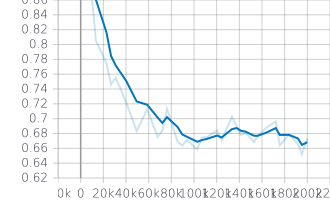
\includegraphics[width=6cm]{./Bilder/eval/loss.png}
        \subcaption{loss}    
    \end{subfigure}
    \caption{Loss und mAP für 200000 Steps}
    \label{plot:map_loss}
\end{figure}


% \begin{figure}[htb]
%     \centering
%     \begin{subfigure}{6cm}
%         \centering
%         \def\svgwidth{5cm}
%         \input{./Bilder/eval/mAP.pdf_tex}
%         %\subcaption{mAP}
%         %\label{subfig:raspy}
%     \end{subfigure}
%     % \begin{subfigure}{6cm}
%     %     \centering
%     %     \def\svgwidth{5cm}
%     %     \input{./Bilder/eval/loss.pdf_tex}
%     %     %\subcaption{Loss}
%     %     %\label{subfig:rpicam}
%     % \end{subfigure}
%     \label{plot:map_loss}
% \end{figure}




% wenn einzelnde klassen evaluiert werden können:
% Spalten: mAP | AP classe1 | AP classe2 | ... | AP classe n



\subsection{Graustufen/Infrarot Bilder}\label{subsec:eval_gray}

Da, wie die Ergebnisse in \ref{subsec:regularization} und 
\ref{subsec:distributions} gezeigt haben eine Augmentierung (welche 
Augmentierungen) die erfogreichste Regularisierungs technik 
war, wurde für die Graustufen Bilder nur Auf Augmentierte Bilder 
mit faster Inception trainiert:
\\
hier für die drei in \ref{subsec:train_gray} verwendeten modelle 
jwls für die in \ref{subsec:distributions} beschriebenen eval daten 
sätze vergleichen.

\begin{table}[htb]
    \centering
    \label{tab:eval_gray}
    \begin{tabular}{| l | l || c | c |} 
        \hline
        Modell & Dataset & mAP & Loss\\
        \hline
        \multirow{2}{*}{rgb} & original & 0.6556 & 0.1451 \\
        & handy & 0.4155 & 0.2389 \\
        \hline
        \multirow{2}{*}{gray 1 channel} & original & 0.5625 & 0.1716 \\
        & handy & 0.3226 & 0.2747 \\
        \hline
        \multirow{2}{*}{gray 3 channel} & original & 0.664 & 0.1653 \\
        & handy & 0.438 & 0.2492 \\
        \hline
    \end{tabular}        
    \caption{Grayscale}
\end{table}


\begin{figure}[htb]
    \centering
    \begin{subfigure}{5cm}
        \centering
        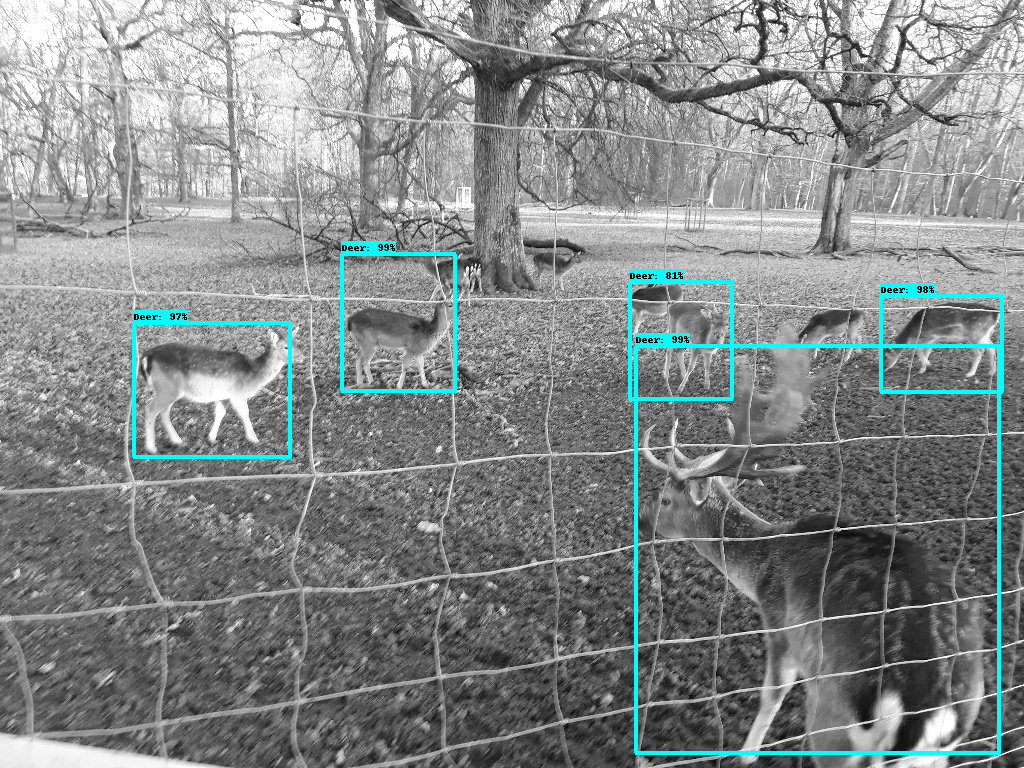
\includegraphics[width=5cm]{./Bilder/eval/rgb.png}
        \subcaption{rbg}
    \end{subfigure}
    \begin{subfigure}{5cm}
        \centering
        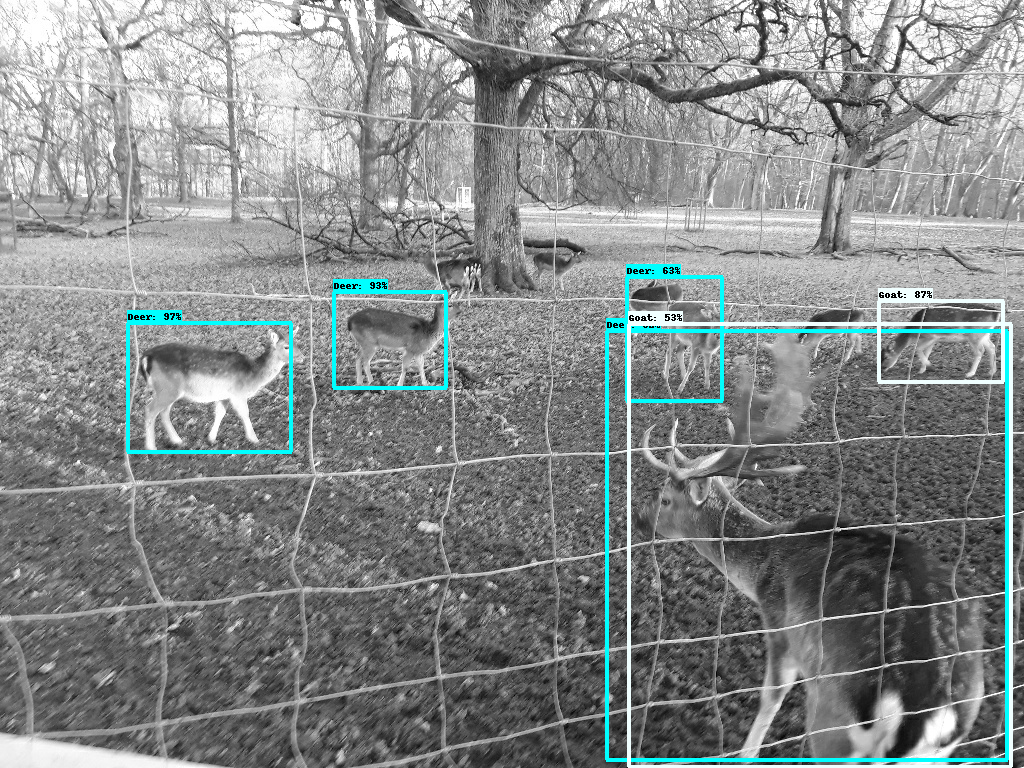
\includegraphics[width=5cm]{./Bilder/eval/gray_1ch.png}
        \subcaption{grau (1channel)}
    \end{subfigure}
    \begin{subfigure}{5cm}
        \centering
        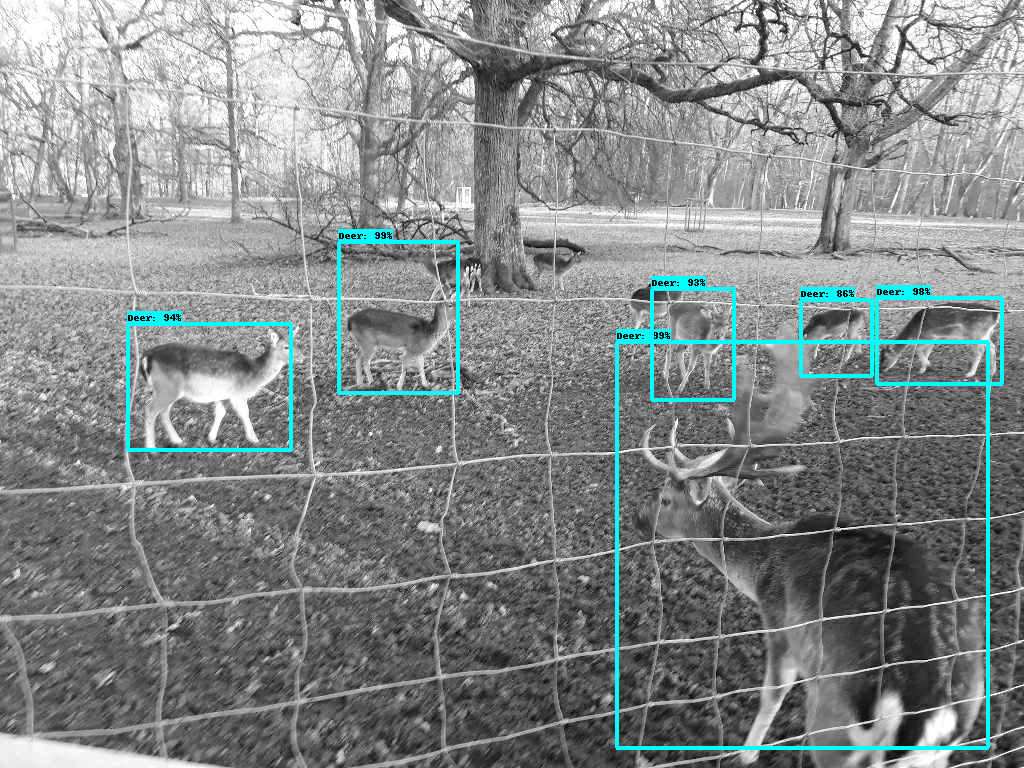
\includegraphics[width=5cm]{./Bilder/eval/gray_3ch.png}
        \subcaption{grau (3channel)}
    \end{subfigure}
    \caption{Vergleich der Inferenz von grau bildern für verschiedene Modelle}
    \label{img:raspy_cam}
\end{figure}





Diskussion des Ergebnisses: welchen einfluss haben Form und Farbe 
bei training, unnötig gelernte features für gray bilder? schnelligkeit?
\\
Da es sich bei den convertierten graustufen bilder ja nicht um 
echte Graustufen bilder handelt, wurden Test Bilder von Alltags gegenständen 
mit der Für die Applikation verwendeten RaspiCam im Infrarot Modus aufgenommen. Um diese 
\\
(hat der Infrarot Modus mit Wärme, also lebendigkeit des Objektes zu zun??)
\\
Um diese Zu testen wurde ein weiteres Netz auf diese Gegenstände 
(Gesicht, Hand, ) trainiert und im folgenden auf 
den Datensatz true-ir evaluiert.

